\documentclass{beamer}
\usepackage{subfig}
\usepackage{amsmath}
\usepackage{bm}
\usepackage[T1]{fontenc}

\DeclareMathOperator*{\argmax}{arg\,max}
\DeclareMathOperator*{\argmin}{arg\,min}


\title{Genetic Algorithms}
\author{Prof. Alessandro Lucantonio}
\institute{Aarhus University}
\date{}

\setbeamertemplate{footline}[frame number]
\setbeamertemplate{navigation symbols}{}


\begin{document}
	\frame{\titlepage}
	
	\begin{frame}
		\frametitle{GA - Main features}
		\begin{itemize}
			\setlength\itemsep{5mm}
			\item Inspired by biological evolution (survival of the fittest, natural selection, and genetic inheritance)
			\item \textbf{Gradient-free}/\textbf{global} optimization
			\item Good choice when the search space is large/multi-dimensional problems
			\item Relatively easy to implement and \textit{parallelize}
		\end{itemize}
	\end{frame}
	

	\begin{frame}
		\begin{figure}
			\centering
			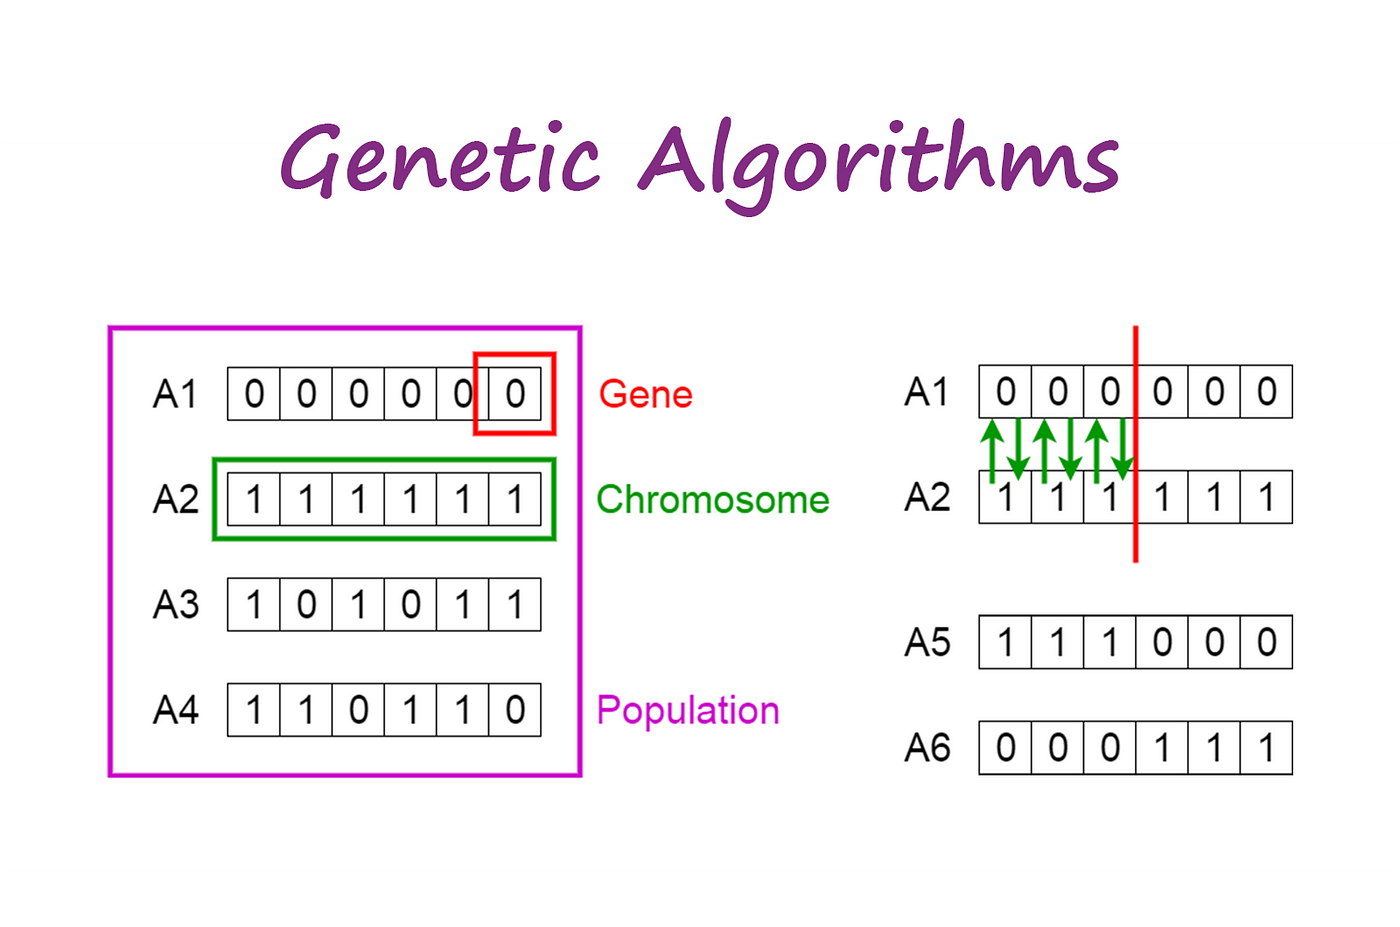
\includegraphics[scale=0.23]{images/ga}
			\caption{Example of binary genes, chromosomes and population in a GA.}
		\end{figure}
	\end{frame}

	

	\begin{frame}
		\frametitle{Basic terminology}
		\begin{itemize}
			\item \textbf{Population}: a collection of candidate solutions
			\item \textbf{Individual}: a candidate solution to the given problem; it is also called \textbf{chromosome}
			\item \textbf{Gene}: the indivisible building block making up an individual
			\item \textbf{Fitness}: a score that measures how good an individual is (as a solution to the given problem)
			\item \textbf{Mutation}: random modification of the genes of an individual
			\item \textbf{Crossover}: combination of the chromosomes of two or more individuals to create a new candidate solution
			\item \textbf{Selection}: choice of individuals to breed the next generation
		\end{itemize}
	\end{frame}

	\begin{frame}
		\frametitle{GA flowchart}
		\begin{figure}
			\centering
			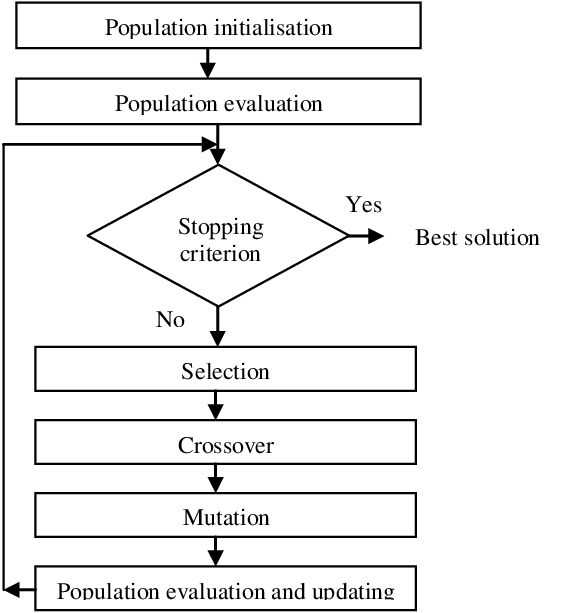
\includegraphics[scale=0.3]{images/ga_scheme}
		\end{figure}
		
	\end{frame}
		
		\begin{frame}
			\frametitle{GA pseudo-code}
			\begin{enumerate}
				\item Randomly generate a population of $m$ parents
				\item Repeat until reaching a stopping criterion
				\begin{enumerate}
					\item Compute the fitness for each individual in the current parent population
					\item Select $p$ parents form the population
					 \item Generate $m$ offspring by crossover
					 \item Probabilistically mutate individuals of the offspring
					 \item Replace the parent population with the offspring
				\end{enumerate}
			\end{enumerate}
			
			\vspace{5mm}
			
			\textit{Note:} the best individuals in the parent population may be lost because the offspring population replaces the parent one (non-monotonic fitness). We can preserve the best using \textbf{elitist selection}.
		\end{frame}
			
			\begin{frame}
				\frametitle{Selection mechanisms}
				
				\textbf{Selection pressure}: greediness or exploitation pressure.
				
				\vspace{5mm}
				
				Some mechanisms ranked from high to low selection pressure:
				\begin{itemize}
					\item \textbf{Tournament}: randomly select $k$ ($k=2,3$, typically) individuals using a uniform probability and then select the best (or worst) individual from the competitors as the winner (or loser). If $p$ individuals need to be selected, $p$ tournaments are performed.
					\item \textbf{Fitness-proportional}: each individual is assigned the probability $f_i/f_{sum}$ where $f_i$ is the fitness of individual $i$ and $f_{sum}$ is the total fitness of all the individuals in the current selection pool 
					\item \textbf{Uniform}: select the parents using a uniform probability distribution
				\end{itemize}
			\end{frame}
			
			\begin{frame}
				\frametitle{Crossover and mutation}
				
				\textbf{Single-point crossover}: call $L$ the number of genes; randomly select a crossover point between genes $i$ and $i+1$ and copy genes $1\dots i$ from parent 1 and genes $i+1...N$ from parent 2.
				\begin{itemize}
					\item Parent 1: A B \textcolor{red}{|} C D E F
					\item Parent 2: a b \textcolor{red}{|} c d e f
					\item Child: A B c d e f
				\end{itemize}
				
				\vspace{5mm}
				
				\textbf{Gaussian mutation}: suppose that the chromosome is made of real numbers; for each gene to be mutated (randomly selected or according to a specific criterion), draw a number from a Gaussian distribution and modify it by adding the extracted number to it.
				
				\vspace{5mm}
				
				Picture an individual as a point in an $N$-dim gene space:  children produced by crossover correspond to vertices of the $N$-dim rectangle defined by the two parents. \textit{Mutation} produces a child by forming a cloud around the parent: it provides a source of useful gene values, while crossover explores the lattice they define.
			
			\end{frame}
			
			\begin{frame}
				\frametitle{GA design - Exploration vs exploitation}
				High-level goal: effective balance between exploration of new regions of the search space and exploitation of the already explored regions.
				
				\vspace{5mm}
				
				\begin{itemize}
					\item \textit{Crossover} and \textit{mutation} are the primary source of \textbf{exploration}, while \textit{selection} controls \textbf{exploitation}
					\item Strong selection pressure should be balanced by more explorative reproductive (crossover/mutation) operators
					\item Size of parent population measures the degree of parallel search (increase for multi-peaked landscapes)
				\end{itemize}
				
			\end{frame}
			
%			\begin{frame}
%				\frametitle{Model Predictive Control - Main features}
%				MPC uses a \textbf{model} of the system to \textbf{predict} future states $x_i \in \mathbb{R}^n$, $i=0,\dots,N-1$ and optimize \textbf{control} inputs $u_i \in \mathbb{R}^m$, $i=0,\dots,M-1$ over a defined \textit{time horizon}.
%				
%				\vspace{5mm}
%				
%				Key components:
%				\begin{itemize}
%				\item \textbf{Predictive Model}: Represents the dynamics of the system (linear/non-linear, discrete/continuous).
%				\item \textbf{Horizon}: Consists of a prediction horizon ($N$ future time-steps) and a control horizon ($M$ future time-steps).
%				\item \textbf{Cost function}: Defined to quantify the desired system performance, typically involves minimizing \textit{error} (of system trajectory with respect to desired/\textit{setpoint} $\bar{x}_i$) and \textit{control effort} (here $N=M$):
%				$$ J = \sum_{i=0}^{N-1}[{s\|x_i - \bar{x}_i\|^2} + q\|u_i\|^2]$$
%				with $s$ and $q$ weights of the cost function terms.
%				\end{itemize}
%		
%				
%			\end{frame}
%			
%		\begin{frame}
%				\frametitle{Model Predictive Control - Algorithm}
%				
%			\begin{columns} 
%				% Column 1
%				\begin{column}{.52\textwidth}
%					Basic steps:
%					\begin{enumerate}
%						\item Measure current state of the system;
%						\item Predict future states $x_i$ using the model;
%						\item Solve an optimization problem to minimize the cost function $J$ with respect to the controls $u_i$, subject to constraints (such as bounds on the controls).
%						\item Apply $u_0$ and go to step 1.
%					\end{enumerate}
%					\vspace{5mm}
%					We can use a \textbf{genetic algorithm} to solve the optimization problem.
%				\end{column}
%				% Column 2    
%				\begin{column}{.52\textwidth}
%					\begin{figure}
%						\centering
%						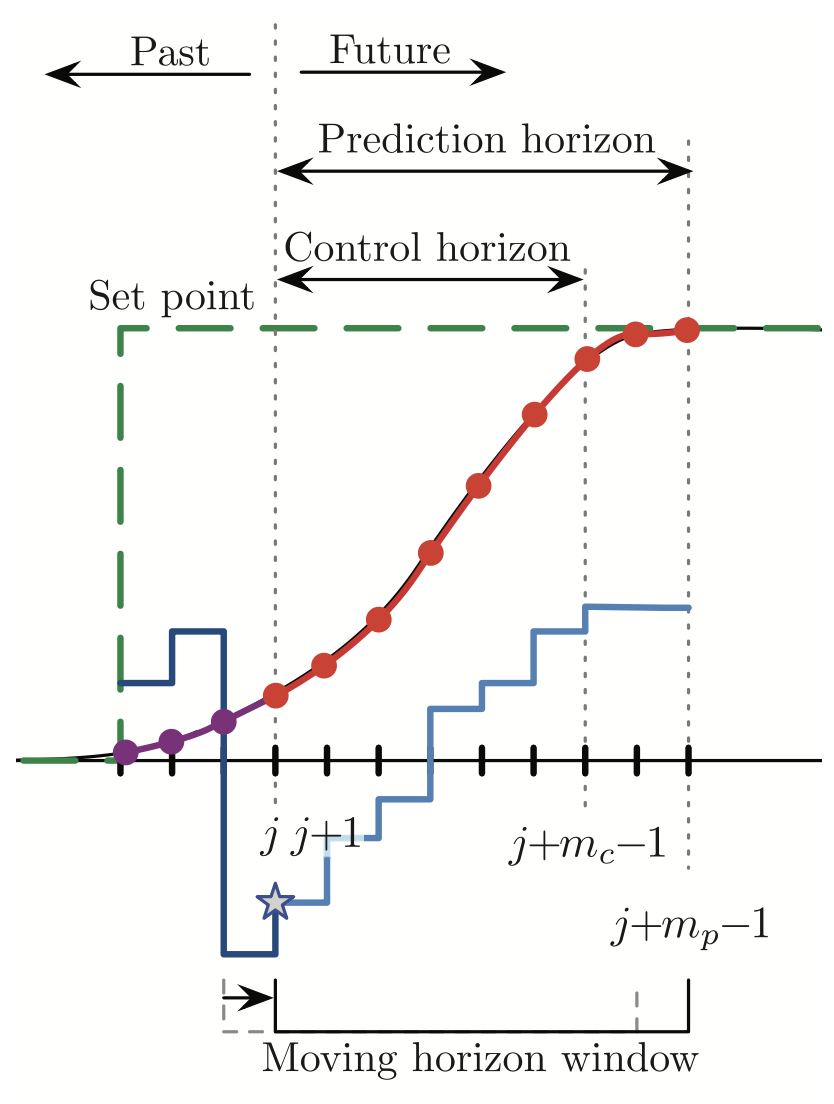
\includegraphics[scale=0.35]{images/mpc_intro}
%						%\caption{}
%						\label{fig:mpcintro}
%					\end{figure}
%				\end{column}
%				
%			\end{columns}
%				
%			
%			
%			
%			
%		\end{frame}
	
\end{document}